% Rešerše – Odoo (vkládá se do kapitoly 01-reserse.tex)
\section{Odoo}\label{sec:reserse-odoo}

Odoo je modulární podnikový systém složený z~desítek aplikací, ze kterých si firma vybírá jen ty, které potřebuje. Základní údaje shrnuje tabulka~\ref{tab:reserse-odoo}.

\begin{table}[H]
\centering
\small
\begin{tabular}{>{\raggedright\arraybackslash}p{0.24\linewidth}>{\raggedright\arraybackslash}p{0.70\linewidth}}
\hline
\textbf{Kritérium} & \textbf{Zjištění} \\
\hline
Název & Odoo (dříve TinyERP a~OpenERP) \\
Společnost & Odoo S.A., Belgie; zakladatel a~generální ředitel Fabien Pinckaers \cite{wiki-odoo,odoo-zdrazeni} \\
Typ aplikace & webová aplikace a~mobilní aplikace \\
Hostování & cloud výrobce (Odoo Online), platforma Odoo.sh i~vlastní server \cite{wiki-odoo,odoo-cenik} \\
Licence & dvě edice: Community jako open-source (LGPLv3), Enterprise jako proprietární předplatné \cite{wiki-odoo,odoo-github} \\
Cena & Community zdarma; v~cloudu je jedna aplikace zdarma s~neomezeným počtem uživatelů; tarif Standardní 11,90~€ (běžně 14,90~€) a~Nestandardní 22,90~€ (běžně 27,90~€) za uživatele a~měsíc; vlastní server, úpravy přes Odoo Studio a~API jen v~tarifu Nestandardní (obrázek~\ref{obr:odoo-cenik}) \cite{odoo-cenik}; implementace u~českých partnerů pro malou firmu přibližně 150 až 400 tisíc~Kč \cite{elfox-odoo} \\
Zkušební verze & 15 dní pro více aplikací, jedna aplikace je zdarma trvale \cite{odoo-cenik} \\
\hline
\end{tabular}
\caption{Základní údaje o~řešení Odoo}\label{tab:reserse-odoo}
\end{table}

\begin{figure}[H]
\centering
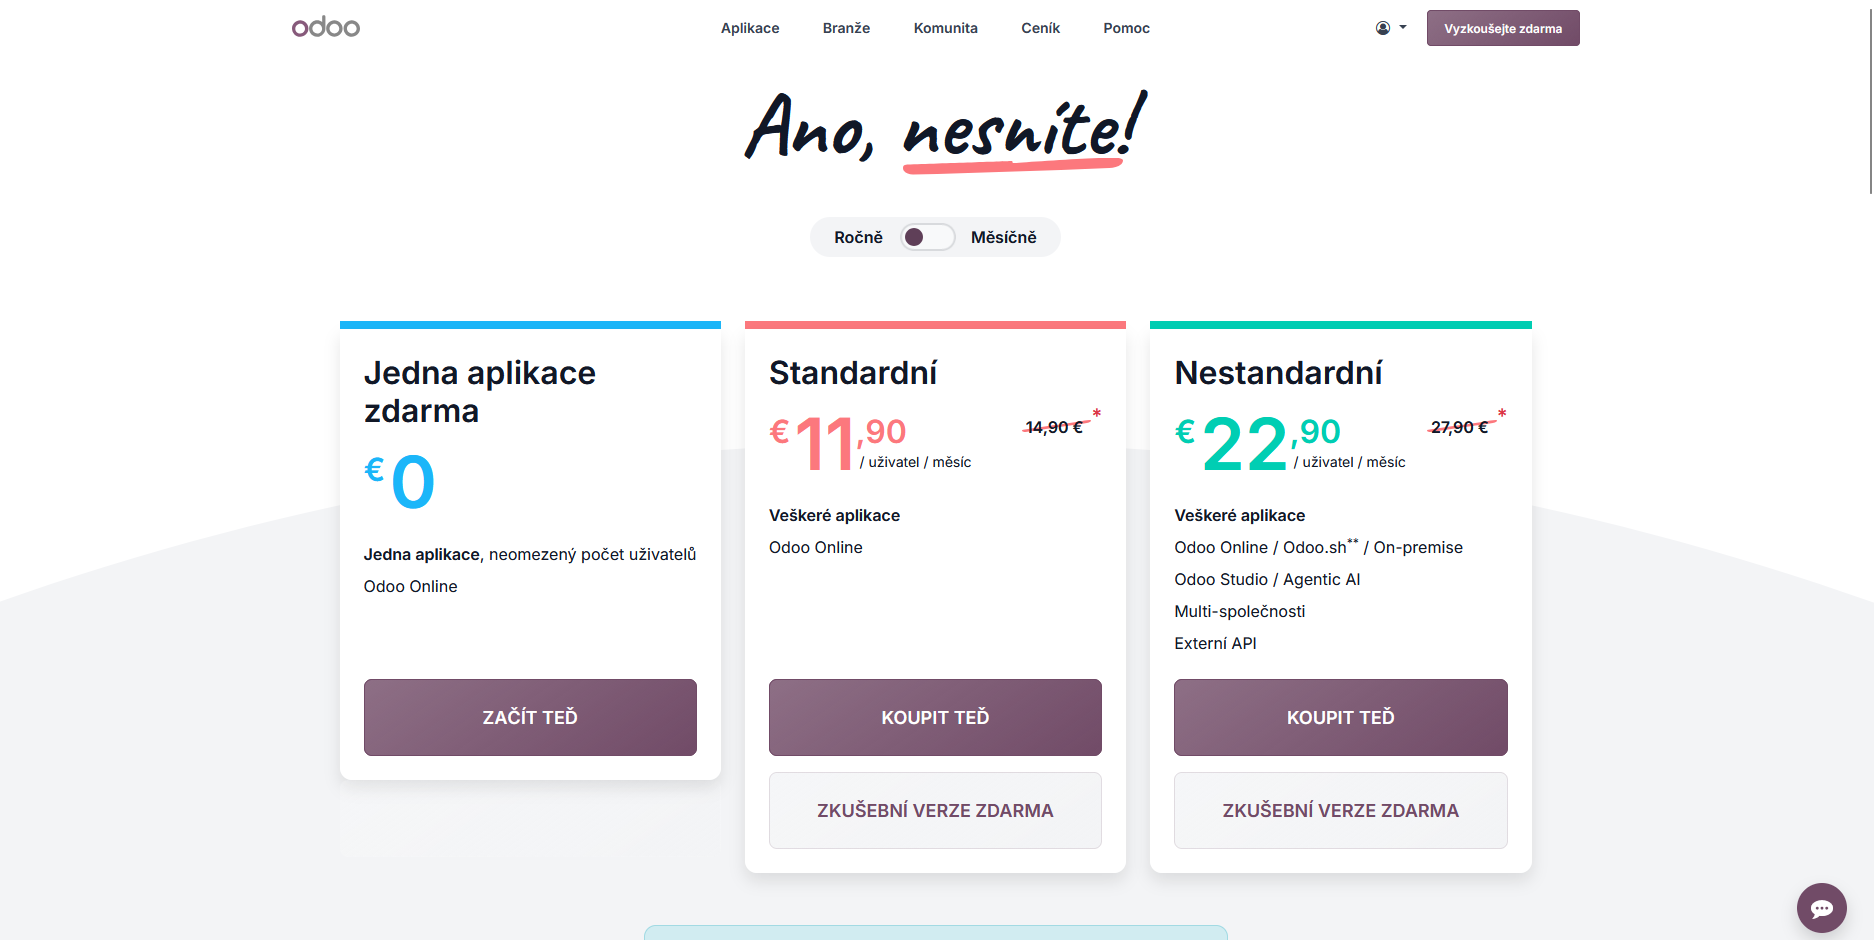
\includegraphics[width=0.9\linewidth]{obrazky/reserse/odoo_cenik_predplatne.png}
\caption{Ceník Odoo pro Českou republiku (zdroj: vlastní snímek obrazovky stránky \protect\url{https://www.odoo.com/cs_CZ/pricing}, pořízeno 3.~11.~2026)}\label{obr:odoo-cenik}
\end{figure}

\subsection{Zkušenosti ze zkušební verze}

Ve zkušební verzi byly vybrány aplikace CRM, Pokladní systém, Fakturace, Dokumenty, Opravy a~Zaměstnanci. Odoo bylo vyzkoušeno jako poslední, protože od něj byl na základě předchozí rešerše očekáván největší přínos. Úvodní obrazovka působí přívětivě: barevné ikony jednotlivých aplikací na tmavém pozadí s~názvy, název firmy a~přihlášený uživatel v~pravém horním rohu. Důležitá tlačítka, například \emph{Nové}, jsou barevně odlišená a~horní lišta ukazuje, ve které části aplikace se uživatel nachází. Tabulky jsou přehledné a~lze je přepnout do zobrazení kanban, seznam, graf nebo kalendář; kanbanové zobrazení kontaktů s~kartami obsahujícími jen základní údaje je velmi přehledné a~je inspirací pro navrhovanou aplikaci. Formulář nového kontaktu má vlevo vstupní pole a~vpravo souhrnný přehled, podobně jako v~navrhované aplikaci, záznam se však ukládá automaticky bez tlačítka \emph{Uložit}, takže uživatel nemá jistotu, zda byl uložen. Stránka Dokumenty se stromem složek je přehledná a~usnadňuje hledání v~uložených souborech. Příjemná je také sekce Aplikace, kde lze aplikace kdykoliv přidat nebo odebrat.

Aplikace Opravy umožňuje založit opravu výrobku i~nový výrobek přímo z~formuláře (obrázek~\ref{obr:odoo-opravy}). Stavy opravy jsou ale jen tři (\emph{Nové}, \emph{Potvrzený} a~\emph{Done}), částečně nepřeložené. Po dokončení opravy lze tlačítkem \emph{Invoice} vytvořit fakturu. Detail faktury nabízí akce Odeslat, Tisk, Zaplatit a~Náhled; tisk však bez náhledu rovnou stáhne soubor PDF a~po jednorázovém výběru vzhledu dokumentu (\emph{Setup your invoice layout}) se možnost jej znovu změnit nepodařilo najít. Nastavit formát číslování dokumentů nelze.

\begin{figure}[H]
\centering
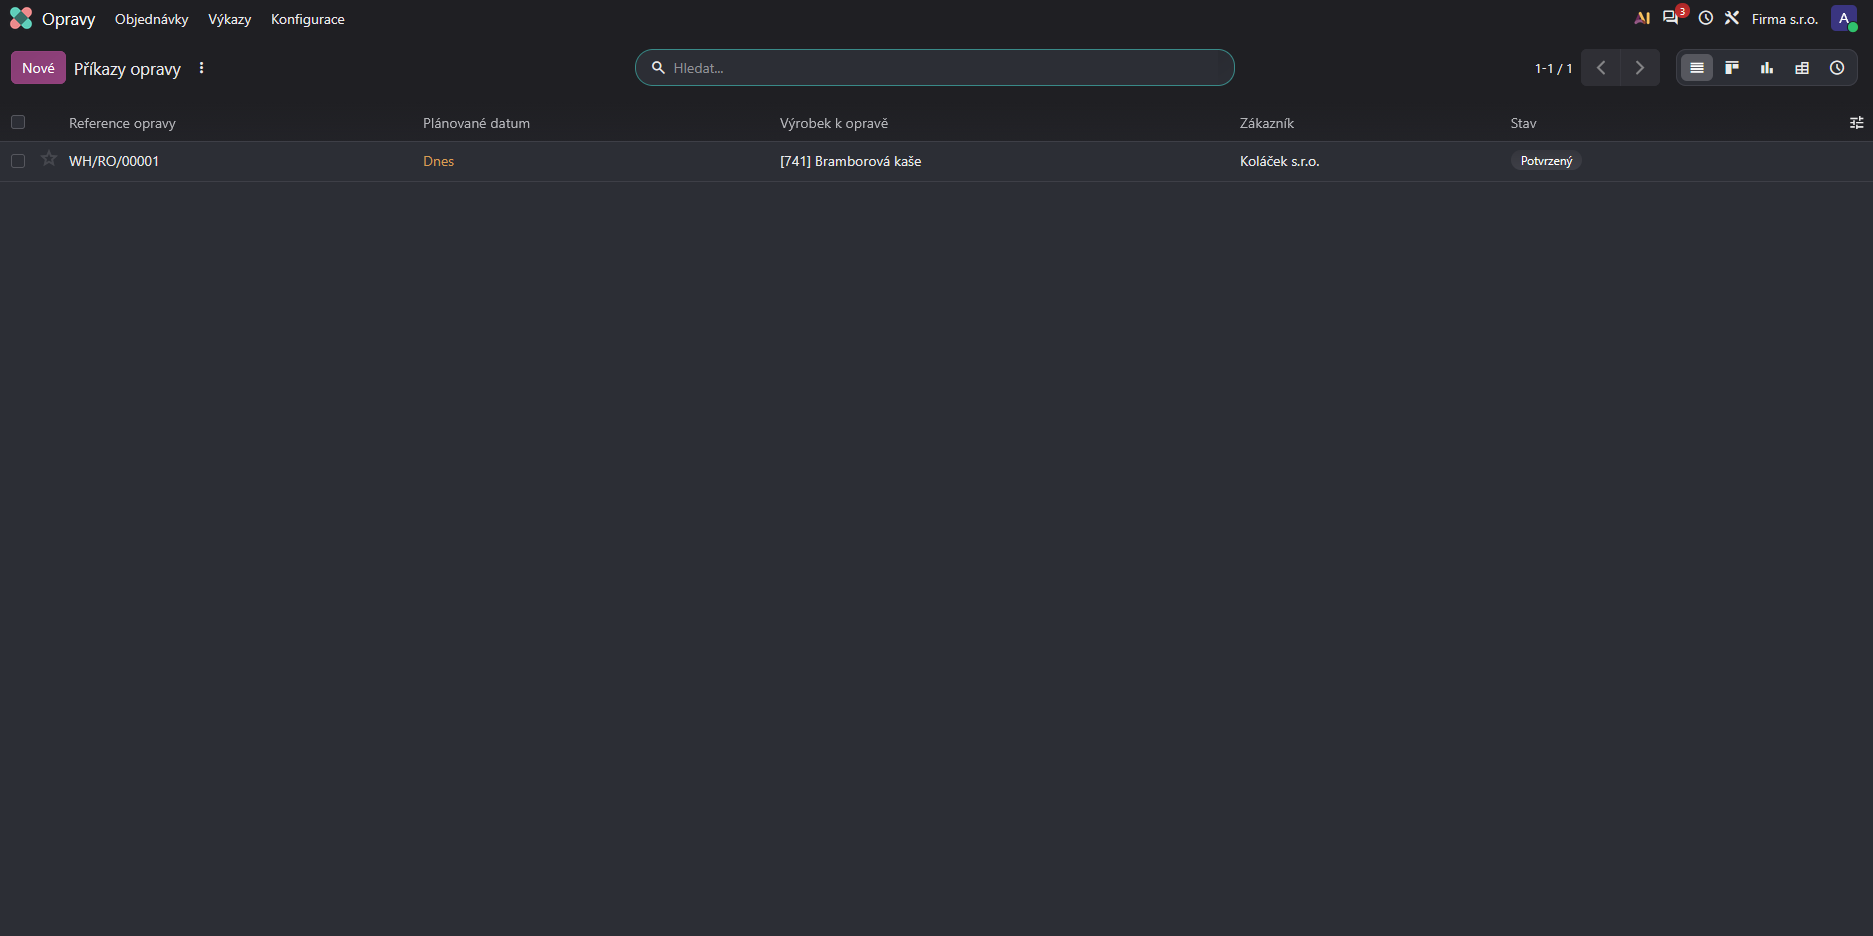
\includegraphics[width=\linewidth]{obrazky/reserse/odoo_strana_opravy.png}
\caption{Seznam oprav v~aplikaci Odoo s~přepínáním zobrazení vpravo nahoře (zdroj: vlastní snímek obrazovky ze zkušební verze, pořízeno 3.~11.~2026)}\label{obr:odoo-opravy}
\end{figure}

Celkový dojem je přesto zklamáním. Navigace je nelogická: odkazy jako \emph{Objednávky} v~aplikaci Opravy vedou na tutéž stránku, \emph{Výkazy} zobrazí jen graf, nabídky jsou skryté pod položkou \emph{Objednávky} a~položky \emph{Zákazníci} a~\emph{Dodavatelé} v~aplikaci Fakturace pouze otevírají další nabídku, takže k~vytvoření faktury vede několik nepřímých kroků. Rozhraní je přeloženo jen částečně, anglické texty se objevují v~tlačítkách i~vstupních polích. Popisky ikon pro přepínání zobrazení se zobrazují pod kurzorem, který je zakrývá. Pravou část každého formuláře zabírá panel s~chatem, historií změn a~aktivitami určený pro spolupráci více zaměstnanců; zabírá téměř polovinu obrazovky, nelze změnit jeho velikost a~pro firmu s~jedním administrativním pracovníkem je zbytečný. Tlačítka \emph{Zrušit} a~\emph{Uložit} v~nastavení bez provedených změn nedělají nic viditelného, chybí tlačítko \enquote{Zpět} (nahrazuje jej jen malý křížek) a~po výběru sekce se nejprve zobrazí přehled s~grafy. Ve srovnání s~navrhovanou aplikací chybí evidence zařízení (aplikace Opravy tento požadavek nesplňuje), servisních zakázek a~provedené práce, materiál je dostupný jen jako součást skladu a~nelze použít vlastní šablony dokumentů.

\subsection{Vhodnost pro malé firmy}

Pokud by firma řešila pouze fakturaci, je Odoo díky trvale bezplatné jedné aplikaci výhodnější než placené fakturační služby. Pro pokrytí potřeb servisní firmy by však musela používat více aplikací v~placeném tarifu za přibližně 12~€ za uživatele měsíčně, a~ani tak by servisní evidence neodpovídala jejím požadavkům. Edice Community je zdarma, ale její provoz na vlastním serveru vyžaduje technické znalosti a~implementace u~partnera se pohybuje ve stovkách tisíc korun. Odoo je tak funkčně silné, ale pro malou servisní firmu provozně i~ekonomicky náročné a~vhodné spíše pro firmy, které počítají s~růstem.
